% (The MIT License)
%
% Copyright (c) 2023-2024 Yegor Bugayenko
%
% Permission is hereby granted, free of charge, to any person obtaining a copy
% of this software and associated documentation files (the 'Software'), to deal
% in the Software without restriction, including without limitation the rights
% to use, copy, modify, merge, publish, distribute, sublicense, and/or sell
% copies of the Software, and to permit persons to whom the Software is
% furnished to do so, subject to the following conditions:
%
% The above copyright notice and this permission notice shall be included in all
% copies or substantial portions of the Software.
%
% THE SOFTWARE IS PROVIDED 'AS IS', WITHOUT WARRANTY OF ANY KIND, EXPRESS OR
% IMPLIED, INCLUDING BUT NOT LIMITED TO THE WARRANTIES OF MERCHANTABILITY,
% FITNESS FOR A PARTICULAR PURPOSE AND NONINFRINGEMENT. IN NO EVENT SHALL THE
% AUTHORS OR COPYRIGHT HOLDERS BE LIABLE FOR ANY CLAIM, DAMAGES OR OTHER
% LIABILITY, WHETHER IN AN ACTION OF CONTRACT, TORT OR OTHERWISE, ARISING FROM,
% OUT OF OR IN CONNECTION WITH THE SOFTWARE OR THE USE OR OTHER DEALINGS IN THE
% SOFTWARE.

\documentclass{article}
\usepackage{../sqm}
\newcommand*\thetitle{Static Analysis}
\begin{document}

\plush{\sqmTitlePage{23}{}}

\qte
  [Steven Johnson]
  {steven-johnson.jpg}
  {\textbf{Lint} is a command which examines C source programs, detecting a number of \ul{bugs} and \ul{obscurities}. It enforces the type rules of C more strictly than the C compilers. It may also be used to enforce a number of \ul{portability restrictions} involved in moving programs between different machines and/or operating systems. Another option detects a number of \ul{wasteful}, or \ul{error prone}, constructions which nevertheless are, strictly speaking, legal.}
  {johnson1977lint}

% Extended static checking for Java

% https://dl.acm.org/doi/pdf/10.1145/1287624.1287633?casa_token=f0xMwXQyTGUAAAAA:9D4WEXeruGVgiyZrUvtOtIw75G4tZJCGDN9wxfRMzVyrsbQHep7Pdzh-QKtKs71zTl-jeGZaaeIXPpQ

\pptBanner{Some Types of Bugs to Be Found by Static Analysis}
\begin{pptWide}{3}
Unreachable Code:
{\small\begin{ffcode}
int a = 10;
if (a > 20) {
  a = a + 1;
}
\end{ffcode}
}\par
Uninitialized Variable:\par
{\small\begin{ffcode}
int x;
int y = x + 42;
print(y);
\end{ffcode}
}

\par\columnbreak\par
Division by Zero:\par
{\small\begin{ffcode}
int f(int x) {
  return 42 / x;
}
\end{ffcode}
}\par
Integer Overflow:\par
{\small\begin{ffcode}
var x: u8 = 142;
x = x * 2;
\end{ffcode}
}
\par\columnbreak\par
Endless Loop:
{\small\begin{ffcode}
int x = 5;
int y = 0;
while (x > 0) {
  y = y + x;
}
\end{ffcode}
}
\end{pptWide}
\plush{}

\qte
  [Brian Chess]
  {brian-chess.jpg}
  {Beware of any tool that says something like, `zero defects found, your program is, rather, now secure.' The appropriate output is, `sorry, \ul{couldn’t find} any more bugs.'}
  {chess2004static}

\pptBanner{False Negative vs. False Positive}
\begin{multicols}{2}
{\small\begin{ffcode}
int f(int x) {
  return 42 / x;
}
\end{ffcode}
}
\par\columnbreak\par
\nospell{\textbf{T}rue \textbf{P}ositive} (TP): \\ ``Division by zero''\par
\nospell{\textbf{F}alse \textbf{P}ositive} (FP): \\ ``Integer overflow''\par
\nospell{\textbf{T}rue \textbf{N}egative} (TN): \\ ``No buffer overflow''\par
\nospell{\textbf{F}alse \textbf{N}egative} (FN): \\ ``No errors at all''\par
\end{multicols}
\plush{}

\plush{\pptBanner{Why do JavaScript developers use linters?}
\begin{itemize}
  \setlength\itemsep{0em}
  \item Prevent Errors
  \item Augment Test Suites
  \item Avoid Ambiguous and Complex Code
  \item Maintain Code Consistency
  \item Faster Code Review
  \item Spare Developers' Feelings
  \item Save Discussion Time
  \item Learn About JavaScript
  \end{itemize}
  \source{tomasdottir2017and}}

\plush{\pptBanner{My Favorite Static Analyzers}
\begin{itemize}
  \item Java:
    \href{https://spotbugs.github.io/}{SpotBugs},
    \href{https://checkstyle.sourceforge.io/}{Checkstyle},
    \href{https://pmd.github.io/}{PMD},
    \href{https://www.qulice.com}{Qulice}\citep{bugayenko2014blog0813} for Java
  \item C++:
    \href{https://clang.llvm.org/extra/clang-tidy/}{Clang-Tidy}
  \item Rust:
    \href{https://github.com/rust-lang/rust-clippy}{clippy}
  \end{itemize}}

\plush{\pptBanner{For some tools you have to pay:}
\begin{itemize}
  \setlength\itemsep{0em}
  \item Coverity by \href{https://scan.coverity.com/}{Synopsys} (US)
  \item Klockwork by \href{https://www.perforce.com/}{Perforce} (US)
  \item Fortify by \href{https://www.microfocus.com/}{Micro Focus} (UK)
  \item \href{https://checkmarx.com/}{Checkmarx} (US)
  \item \href{https://www.veracode.com/}{Veracode} (US)
  \item \href{https://snyk.io/}{Snyk} (US)
  \item \href{https://pvs-studio.com/en/pvs-studio/}{PVS-Studio} (Russia)
  \end{itemize}}

\pitch{
  \pptBanner{SARIF}
  \begin{multicols}{2}
  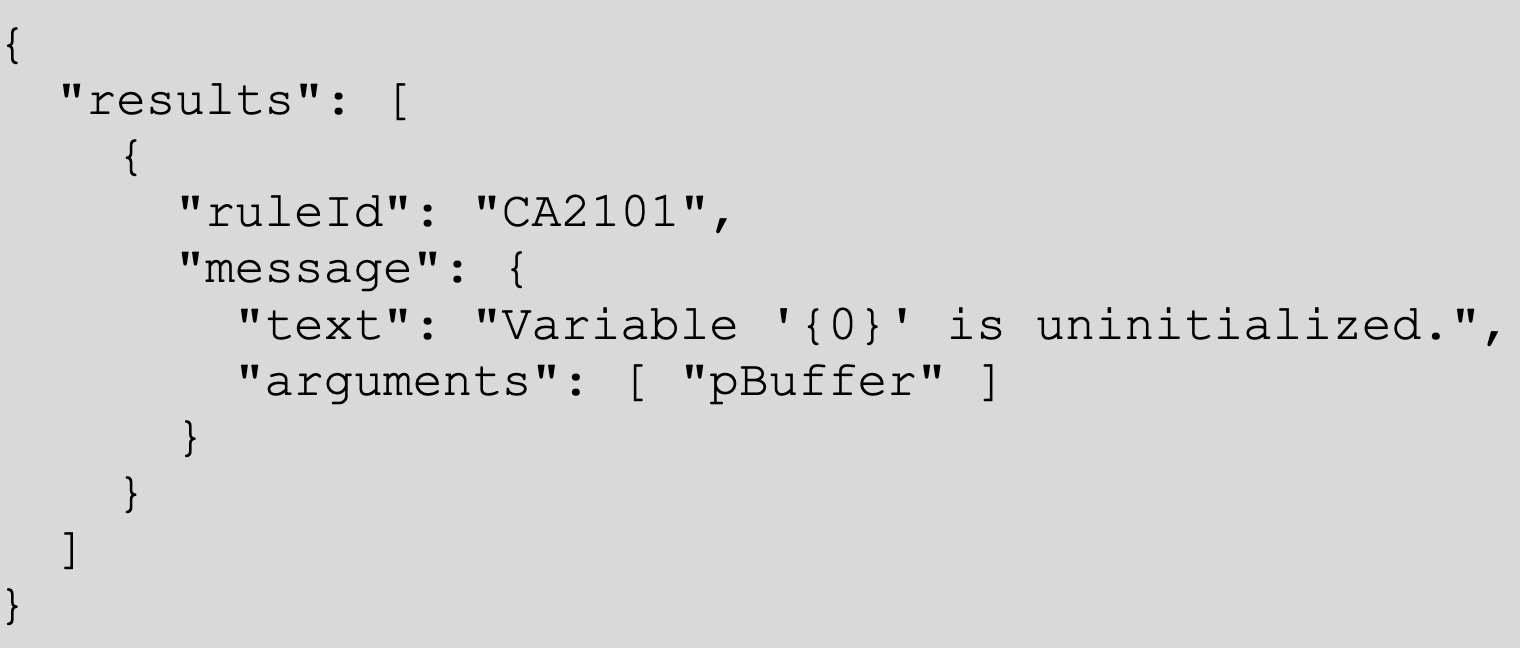
\includegraphics[width=.95\linewidth]{sarif.png}
  \par\columnbreak\par
  ``This document defines a standard format for the output of static analysis tools.''
  \source{sarif2023}
  \end{multicols}}

\qte
  [\nospell{Krist{\'\i}n Fj{\'o}la T{\'o}masd{\'o}ttir}]
  {kristin-tomasdottir.jpg}
  {Every single interview participant mentioned that one of the reasons why they use a linter is to maintain code \ul{consistency}.}
  {tomasdottir2018adoption}
\pitch{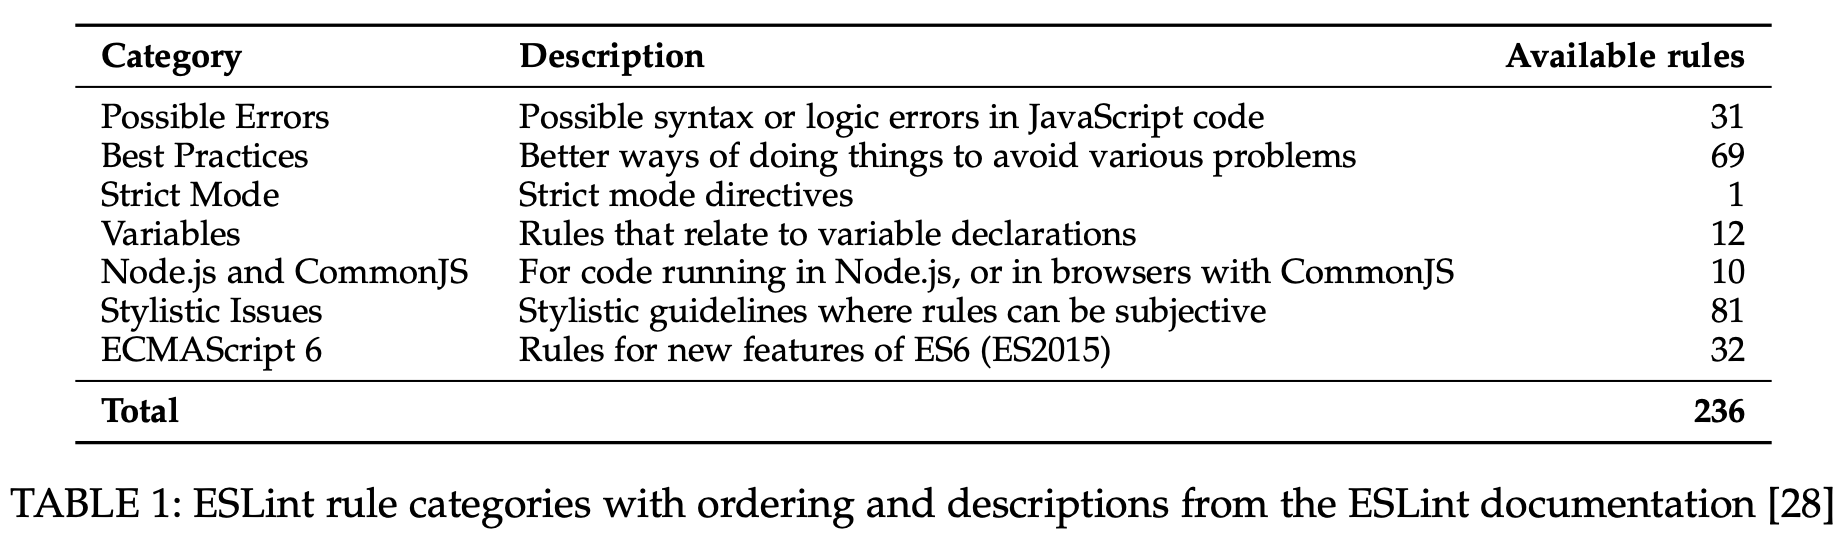
\includegraphics[width=.95\linewidth]{rules.png}
  \source{tomasdottir2018adoption}}

\qte
  [\nospell{Florian Oberm{\"u}ller}]
  {florian-obermuller.jpg}
  {We introduce the concept of \ul{code perfumes} as the counterpart to \ul{code smells}, indicating the correct application of programming practices considered to be good. Using a catalogue of 25 code perfumes for, we empirically demonstrate that these represent frequent practices in, and we find that better programs indeed contain more code perfumes.}
  {obermuller2021code}


\end{document}
